\documentclass[border=12pt]{standalone}
\def\pgfsysdriver{pgfsys-dvisvgm.def}
\usepackage[dvisvgm]{xcolor}
\usepackage{xeCJK}
\setCJKmainfont{HaranoAjiGothic-Regular.otf}[BoldFont=HaranoAjiGothic-Bold.otf]
\setCJKsansfont{HaranoAjiGothic-Regular.otf}[BoldFont=HaranoAjiGothic-Bold.otf]
\usepackage{amsmath,amssymb,tikz,lmodern}
\usetikzlibrary{arrows.meta,positioning,calc,fit,backgrounds}
\renewcommand{\familydefault}{\sfdefault}
\definecolor{ink}{HTML}{25322F}
\definecolor{green}{HTML}{246657}
\definecolor{tint}{HTML}{EEF4F0}
\definecolor{soft}{HTML}{C6D2CC}
\definecolor{muted}{HTML}{52615B}
\newif\ifJapanese
\newcommand{\Tx}[2]{\ifJapanese #1\else #2\fi}
\newcommand{\Eff}{\overline{\operatorname{Eff}}}
\newcommand{\heading}[3]{{\color{green}\bfseries #1\quad\Tx{#2}{#3}}\\[5pt]}
% A white rectangle makes the complete citation label clickable, including spaces.
\newcommand{\refurl}[2]{\special{dvisvgm:raw <a xlink:href="#1" target="_blank" rel="noopener noreferrer">}{\setlength{\fboxsep}{0pt}\colorbox{white}{\color{green}\underline{\strut #2}}}\special{dvisvgm:raw </a>}}
\tikzset{
 card/.style={draw=soft,fill=white,rounded corners=2pt,align=left,text=ink,font=\fontsize{10.5}{14}\selectfont,inner xsep=12pt,inner ysep=10pt,text width=16cm},
 half/.style={card,text width=7.1cm,minimum height=2.05cm},
 result/.style={draw=green,fill=tint,line width=.9pt},
 reason/.style={align=left,text=muted,font=\fontsize{9}{12}\selectfont,inner sep=0pt,text width=14.3cm},
 branchreason/.style={reason,text width=6.4cm},
 edge/.style={-{Stealth[length=2.4mm]},draw=green,line width=1pt},
 wire/.style={draw=green,line width=1pt},
}
% Keep the arrow in a dedicated left gutter; explanations never cover it.
\newcommand{\flow}[3]{
 \coordinate (#2-from) at ($(#1.south)+(-7.7,0)$);
 \coordinate (#2-to) at ($(#2.north)+(-7.7,0)$);
 \draw[edge] (#2-from)--(#2-to);
 \node[reason,anchor=west] (#2-reason) at ($(#2-from)!.5!(#2-to)+(.55,0)$) {#3};
}

\newcommand{\RA}[1]{\refurl{\sourceRA}{#1}}
\newcommand{\OI}[1]{\refurl{\sourceOI}{#1}}
\newcommand{\FF}[1]{\refurl{\sourceFF}{#1}}
\newcommand{\FFcor}[1]{\refurl{\sourceFFcor}{#1}}
\newcommand{\BBT}[1]{\refurl{\sourceBBT}{#1}}
\newcommand{\FG}[1]{\refurl{\sourceFG}{#1}}
\newcommand{\CP}[1]{\refurl{\sourceCP}{#1}}
\newcommand{\BDPP}[1]{\refurl{\sourceBDPP}{#1}}
\newcommand{\pe}{\mathrel{\geq_{\mathrm{pe}}}}
\newcommand{\rowflow}[3]{
 \coordinate (#2-a) at ($(#1.south)+(-3.45,0)$);
 \coordinate (#2-b) at ($(#2.north)+(-3.45,0)$);
 \draw[edge] (#2-a)--(#2-b);
 \node[branchreason,anchor=west] at ($(#2-a)!.5!(#2-b)+(.45,0)$) {#3};
}

\newcommand{\sourceRA}{https://github.com/openai/math/blob/fd4aeeb2ee4fc729c18d98444fed42fd0529eeeb/preprints/The-reverse-logarithmic-Kodaira-inequality-and-additivity-September-26-2026/paper.pdf}
\newcommand{\sourceOI}{https://github.com/openai/math/blob/fd4aeeb2ee4fc729c18d98444fed42fd0529eeeb/preprints/Orbifold-and-logarithmic-Iitaka-subadditivity-September-26-2026/paper.pdf}
\newcommand{\sourceFF}{https://www.math.kyoto-u.ac.jp/~fujino/vmhs-sp108.pdf}
\newcommand{\sourceFFcor}{https://www.math.kyoto-u.ac.jp/~fujino/fujino-fujisawa-memo2.pdf}
\newcommand{\sourceBBT}{https://arxiv.org/pdf/1811.12230v3}
\newcommand{\sourceFG}{https://www.numdam.org/item/10.5802/aif.2894.pdf}
\newcommand{\sourceCP}{https://arxiv.org/pdf/1508.02456v4}
\newcommand{\sourceBDPP}{https://arxiv.org/pdf/math/0405285v1}
\Japanesetrue
\begin{document}
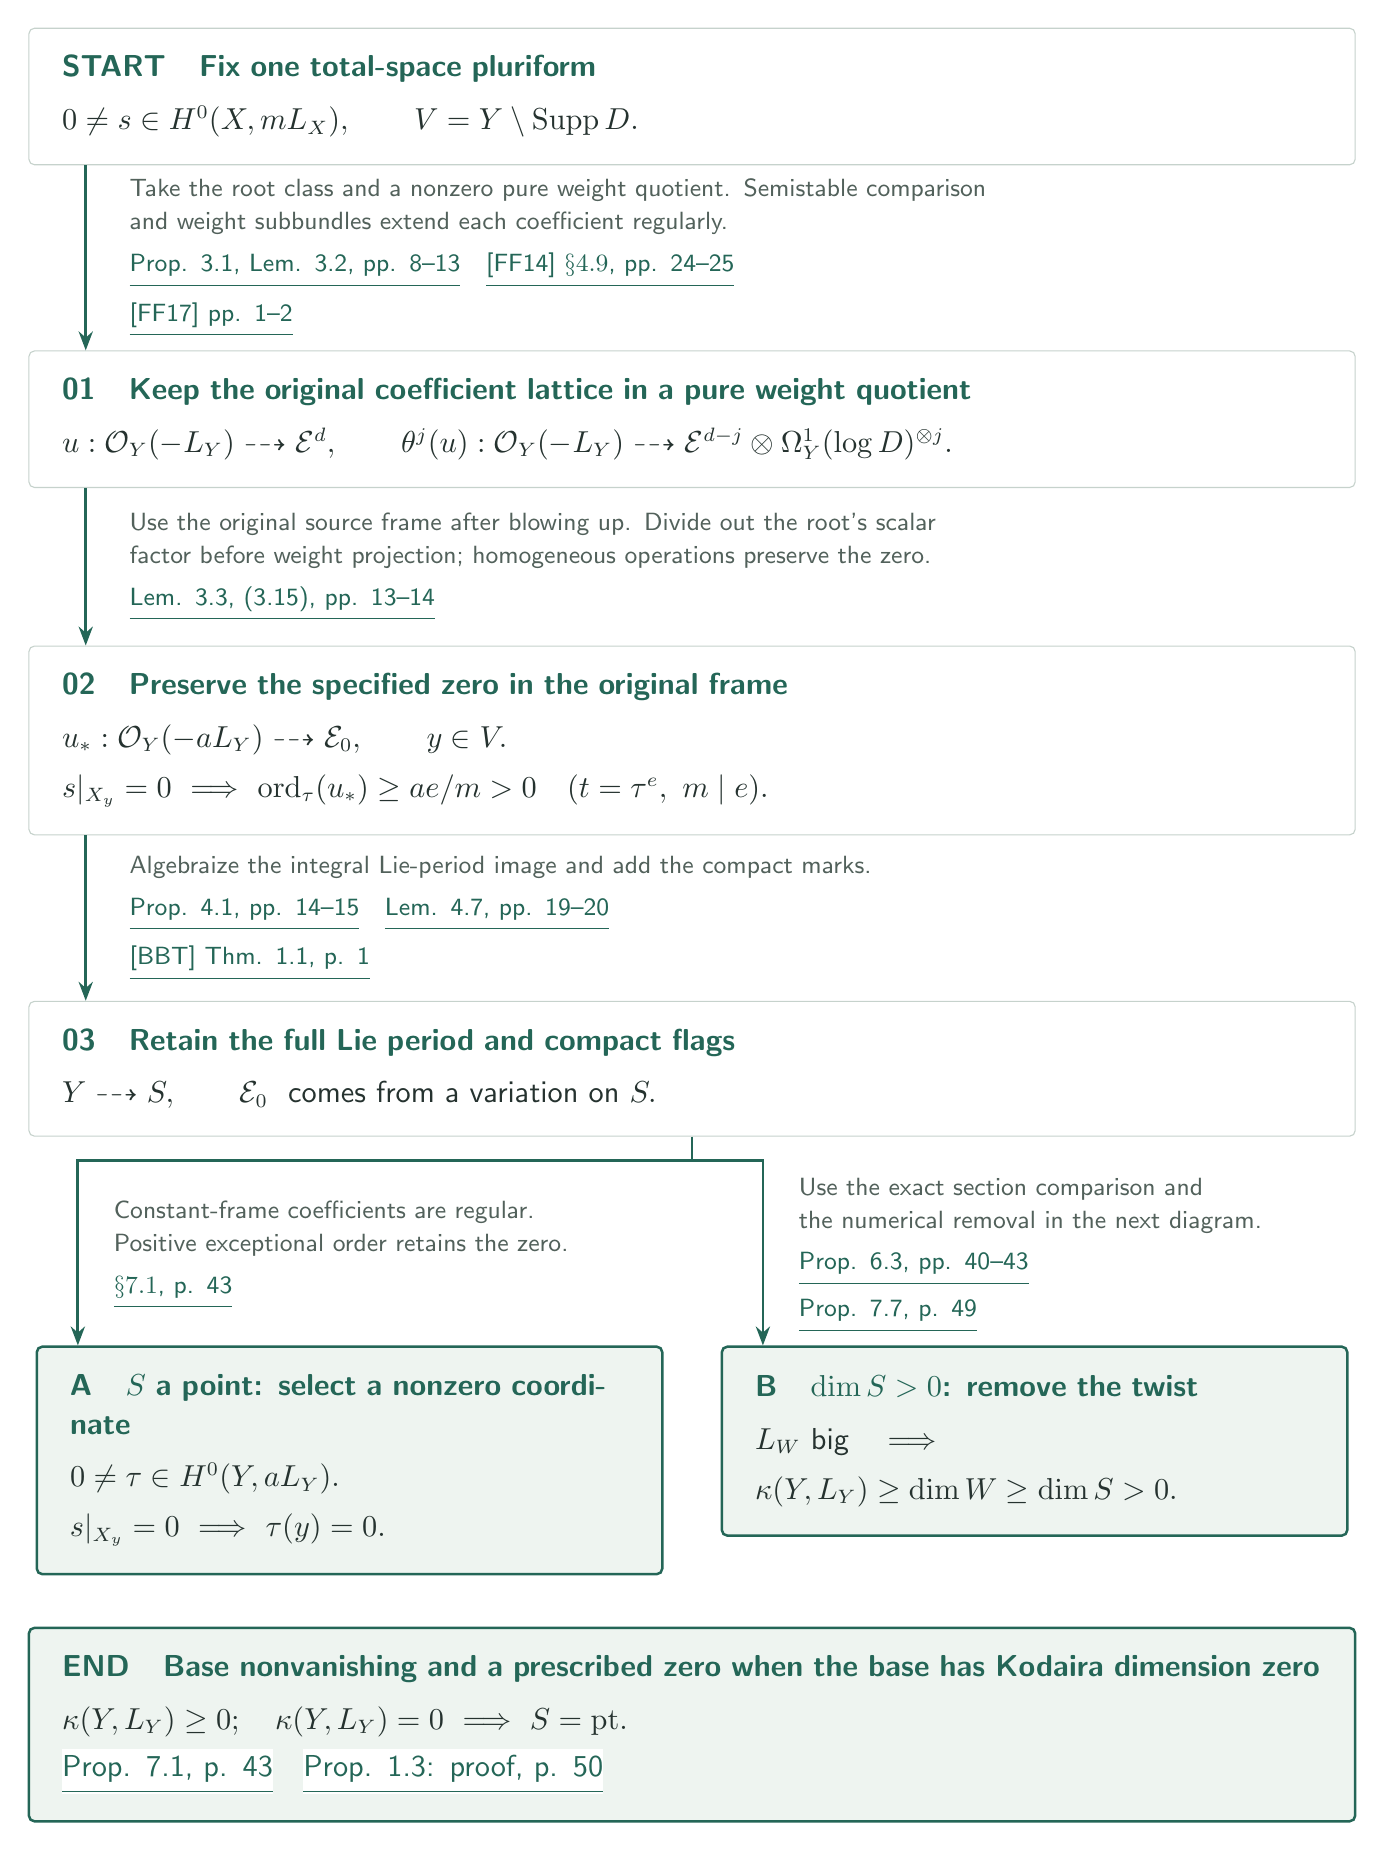
\begin{tikzpicture}
\node[card] (s) {\heading{START}{全空間の一つのpluriformを固定する}{Fix one total-space pluriform}
$0\ne s\in H^0(X,mL_X),\qquad V=Y\setminus\operatorname{Supp}D.$};
\node[card,below=2.35cm of s] (u) {\heading{01}{純weight商で元の係数格子を保持する}{Keep the original coefficient lattice in a pure weight quotient}
$u:\mathcal O_Y(-L_Y)\dashrightarrow\mathcal E^d,\qquad
\theta^j(u):\mathcal O_Y(-L_Y)\dashrightarrow\mathcal E^{d-j}\otimes\Omega_Y^1(\log D)^{\otimes j}.$};
\flow{s}{u}{\Tx{巡回被覆の根をHodge類へ移し、非零の純weight商を取る。\\半安定比較と部分束性により、各係数が正則に延長する。}{Take the root class and a nonzero pure weight quotient. Semistable comparison\\and weight subbundles extend each coefficient regularly.}\\[3pt]
\RA{Prop. 3.1, Lem. 3.2, pp. 8--13}\quad\FF{[FF14] $\S4.9$, pp. 24--25}\\[3pt]
\FFcor{[FF17] pp. 1--2}}
\node[card,below=2cm of u] (zero) {\heading{02}{指定点の零点を元の枠で保持する}{Preserve the specified zero in the original frame}
$u_*:\mathcal O_Y(-aL_Y)\dashrightarrow\mathcal E_0,\qquad y\in V.$\\[4pt]
$s|_{X_y}=0\ \Longrightarrow\ \operatorname{ord}_{\tau}(u_*)\geq ae/m>0\quad(t=\tau^e,\ m\mid e).$};
\flow{u}{zero}{\Tx{blowup後も元のsource lineを使う。根の因子を割り出してから\\weight商へ射影し、斉次テンソル操作で零点を保つ。}{Use the original source frame after blowing up. Divide out the root's scalar\\factor before weight projection; homogeneous operations preserve the zero.}\\[3pt]\RA{Lem. 3.3, (3.15), pp. 13--14}}
\node[card,below=2.1cm of zero] (quotient) {\heading{03}{全Lie periodとcompact flagを記録する}{Retain the full Lie period and compact flags}
$Y\dashrightarrow S,\qquad\mathcal E_0\ \Tx{\text{ は }S\text{ 上の変動から来る。}}{\text{ comes from a variation on }S.}$};
\flow{zero}{quotient}{\Tx{格子を保持した全Lie period像を代数化し、compact markを加える。}{Algebraize the integral Lie-period image and add the compact marks.}\\[3pt]\RA{Prop. 4.1, pp. 14--15}\quad\RA{Lem. 4.7, pp. 19--20}\\[3pt]\BBT{[BBT] Thm. 1.1, p. 1}}
\node[half,result,below=2.65cm of quotient.south,anchor=north,xshift=-4.35cm,minimum height=2.4cm] (point) {\heading{A}{$S$が点：非零の定数座標を選ぶ}{$S$ a point: select a nonzero coordinate}
$0\ne\tau\in H^0(Y,aL_Y).$\\[4pt]
$s|_{X_y}=0\ \Longrightarrow\ \tau(y)=0.$};
\node[half,result,below=2.65cm of quotient.south,anchor=north,xshift=4.35cm,minimum height=2.4cm] (positive) {\heading{B}{$\dim S>0$：捻りを除く}{$\dim S>0$: remove the twist}
$L_W\ \text{big}\quad\Longrightarrow$\\[4pt]
$\kappa(Y,L_Y)\geq\dim W\geq\dim S>0.$};
\draw[wire] (quotient.south)--++(0,-.3) coordinate (fork);
\draw[edge] (fork)-|($(point.north)+(-3.45,0)$);
\draw[edge] (fork)-|($(positive.north)+(-3.45,0)$);
\node[branchreason,anchor=west] at ($(point.north)+(-3,1.15)$) {\Tx{定数枠の係数は全素因子で正則。\\正の例外次数が元の点での零点を与える。}{Constant-frame coefficients are regular.\\Positive exceptional order retains the zero.}\\[3pt]\RA{$\S7.1$, p. 43}};
\node[branchreason,anchor=west] at ($(positive.north)+(-3,1.15)$) {\Tx{相対飯高の完全切断空間の比較と、\\次図の数値的除去を使う。}{Use the exact section comparison and\\the numerical removal in the next diagram.}\\[3pt]\RA{Prop. 6.3, pp. 40--43}\\[2pt]\RA{Prop. 7.7, p. 49}};
\node[card,result,below=.65cm of point.south,anchor=north,xshift=4.35cm] (end) {\heading{END}{非消滅と、小平次元0の場合の指定点の零点}{Base nonvanishing and a prescribed zero when the base has Kodaira dimension zero}
$\kappa(Y,L_Y)\geq0;\quad\kappa(Y,L_Y)=0\ \Longrightarrow\ S=\mathrm{pt}.$\\[3pt]
\RA{Prop. 7.1, p. 43}\quad\RA{Prop. 1.3: proof, p. 50}};
\end{tikzpicture}

\end{document}
